\section{Paradigms in data structuring}
\label{sec:paradigms}

The contemporary meaning of \Term{paradigm} was introduced by
\textcite{Kuhn1962} in the history of science. He explained fundamental changes
in science, like the Copernican Revolution and \person[Albert]{Einstein}'s
theories of relativity as shifts in scientific paradigm. A paradigm is ``what
members of a scientific community, and they alone, share'' \cite{Kuhn1974},
especially their basic theories, assumptions, and research methods. The term is
now also used in a broader sense for ``a philosophical or theoretical framework
of any kind'' \cite{Webster2011}. Paradigms are relevant to analysis of data
structuring methods, because they deeply shape the way people talk and think
about data. Paradigms in data structuring, however, differ from scientific
paradigms, because data structuring and description is more art and engineering
practice than science \cite{Simsion2007}.  One can identify some paradigm
shifts in the history of data structuring \cite[to give some
examples]{Codd1970,Chen1976,Gamma1994}, but these shifts are less complete and
disruptive for data applications as a whole. The reason is that there is less
ambition to create one single method to structure and describe all data.
Instead it is usual to have many specialized technologies for different use
cases, each based on some paradigm and shared by its own community. So the
following paradigms do not deal with concrete and influential trends like the
\term{relational database model} or the \term{Resource Description Framework}.
They rather describe general kinds of viewing at and dealing with data and with
digital documents. These orthogonal perceptions of data come with their own
basic and often hidden assumptions.  More subliminal than concrete
technologies, paradigms in data structuring influence which patterns are used
as constituent primitives and which are ignored. Five groups of paradigms are
exposed below, each with strengths, weaknesses and related data patterns at the
end of each section.

\begin{itemize}
\item Documents and objects (section~\ref{sec:docobj}) realize digital documents 
  as given or as created artifacts.

\item Standards and rules (section~\ref{sec:standardsrules}) specify the consistent
  creation and consumption of data. They show which parts of a document are 
  possible and relevant and how to make use of data.

\item Collections, types and sameness (section~\ref{sec:collectionstopic}) group
  parts of digital documents based on their identities.

\item Entities and connections (section~\ref{sec:entcon}) seem to be basic 
  building blocks of all, but they are two sides of the same coin.

\item Levels of abstraction (section~\ref{sec:levels})
  separate and combine descriptions of the 
  same document with different granularity.
\end{itemize}


% 1 %%%%%%%%%%%%%%%%%%%%%%%%%%%%%%%%%%%%%%%%%%%%%%%%%%%%%%%%%%%%%%%%%%%%%%%%%%%
\subsection{Documents and objects}
\label{sec:docobj}

The primary question when encountering a piece of data is ``what is this
digital piece and how can it be described?''.  Documents and objects are two
rivaling approaches to describe digital artifacts, answering the question from
two points of view (\ref{sec:tpow}). Both views will be illustrated with examples
(\ref{sec:docobjex}) before uniting them as two sides of the coin of data as sign
(\ref{sec:dataassign}).

\subsubsection{Two points of view}
\label{sec:tpow}

The \term[document!as paradigm to describe data]{document} view primarily tries
to describe the artifact in more or less detail. For instance a document can be
described by its format, size, and divisions. One can model the document, for
instance as \term[ordered hierarchy of content objects]{ordered hierarchy}, and
express it, for instance in a \term{markup language} such as \acro{TEI}. Even
alternative descriptions are possible, for instance concurrent hierarchies
\cite{Renear1996,Pondorf2010}, as long as all descriptions are discoveries of
the same concrete document. The object point of view, in contrast, is less
interested in the specific details of form: it rather tries to create a broad
picture of the document content. An example of the object view is a description
of data as set of connected entities and properties. The document approach is
mainly found in library information science where cataloging is applied to
document artifacts that (are assumed to) already exist. The second approach is
mainly found in computer science and in software engineering where digital
artifacts are created to solve tasks of computation. 
Both views, however, always exist together. Neither documents nor objects are
better descriptions per se, but both are valid, and both can be found on a
large scale and on a small scale. The important question to reveal this
paradigm is not whether data is better described as documents or as objects,
but where a line between the two is drawn in a particular (application of) data
technology. 

\subsubsection{Examples}
\label{sec:docobjex}

A visible instance of this separation is the distinction between
data values and data objects, for instance in databases and in modeling
languages.  Example~\ref{ex:ormsql} shows a simple \acro{ORM} data model and a
corresponding \acro{SQL} schema with years, events, places, and names. Years
and names are defined as values types in the model, so they are given directly
in concrete model instances. Places and events, in contrast, are abstract
entity types which are objects without explicit form.  In the \term{SQL
schema} values are expressed by fields with data types, and objects are
expressed by tables.  Still, objects cannot exist alone, but they need data
fields that act as object place-holders, such as the \sql{Id} fields in
example~\ref{ex:ormsql}. The difficult task is to find out which parts of data
are plain documents, and which parts are arbitrary object identifiers.

\begin{example}
\begin{tikzpicture}[orm]
\entity (e) {Event};
\roles (r) [left=of e,unique=2] {};
\plays[mandatory] (e) to (r);
\value[left=of r] (y) {Year} edge[plays] (r);
\roles (ep) [right=of e] {} edge[plays,unique=1] (e);
\entity (p) [right=of ep] {Place};
\plays (p) to (ep);
\roles (r)  [right=of p,unique=1,unique=2] {} edge[plays,required by] (p);
\value[right=of r] (y) {Name} edge[plays] (r);
\end{tikzpicture}

\begin{lstlisting}[language=SQL]
CREATE TABLE Event (
  Id      int  PRIMARY KEY IDENTITY,
  YearAD  int  NOT NULL,
  PlaceId int,
  FOREIGN KEY (PlaceId) REFERENCES Place(Id)
);
CREATE TABLE Place (
  Id      int  PRIMARY KEY IDENTITY,
  Name    char UNIQUE NOT NULL
);
\end{lstlisting}
\caption{Documents as values and objects as entities/tables in \acrostyle{ORM} and \acrostyle{SQL}}
\label{ex:ormsql}
\end{example}

The line between documents and objects is often less clear than the distinction
between value types or field values, and entity types or object identifier in
example~\ref{ex:ormsql}. As described in section~\ref{sec:descrids},
identifiers can also hold information about the objects they refer to --- in
this case data objects are values. In the same way, most document
values can be interpreted as \term{descriptive identifier}s for some objects:
for instance the \sql{YearAD} field in example~\ref{ex:ormsql} may not only
hold a year number but refer to another table that describes Years objects.
Both variants can better be shown in \acro{RDF} which has a clear separation
between resources as objects on the one side and literals on the
other.\footnote{A parallel document/object dichotomy in \acro{RDF} exists with
the separation between \term{information resource}s and \term{non-information
resource}s \cite{Ayers2008}.} In \acro{RDF} years are normally be expressed as
literals with datatype \rdf{xs:integer} or \rdf{xs:gYear}.  But in some data
sets years are objects, identified by \term{URI reference}s, such as
\rdf{<http://dbpedia.org/resource/2010>} for the year 2010. The choice is
rather arbitrary from a conceptual perspective, but \acro{RDF} technologies
provide no mechanism to switch between document form and object form. A
possible mapping in extended \acrostyle{RDF} would be the Turtle statement

\begin{lstlisting}[language=turtle] 
 "2010"^^xs:gYear owl:sameAs <http://dbpedia.org/resource/2010> . 
\end{lstlisting} 

\noindent but no common \acro{RDF} software can make sense of this.\footnote{In
an April Fool's joke \textcite{Vrandecic2010} provided a similar mapping
between numbers as values and numbers as resources. There is some awareness of
the dichotomy between documents and objects, but crossing the line in practice
seems to be no serious option.}

Switching between data as document and data as object is also possible for
non-descriptive identifiers.  As shown in example~\ref{ex:isbns}, an
\acro{ISBN} can be expressed in several variants (\acro{ISBN}-10,
\acro{ISBN}-13, with/without hyphen or space, etc.). While a general
\acro{ISBN} is an identifier that refers to an abstract publication object,
each variant is a distinct document.  Another example are number encodings
(section~\ref{sec:numberencodings}) which treat numbers as abstract objects
while they are used as concrete values in other context. Number encodings are
just one instance of datatypes (section~\ref{sec:datatypes}), which are used to
tag data pieces as values.  One can also find document values combined with the
entities and relationships paradigm where objects are seen as as primary
objects and values are attached to objects as secondary `properties' or
`attributes' (paradigm~\ref{sec:entcon}).  As discussed in
paradigm~\ref{sec:levels}, levels of abstraction can act as borders between the
two forms of a piece of data.

\subsubsection{Data as sign}
\label{sec:dataassign}

Actually both approaches are two sides of a coin: the document may {\em
contain} an object and the object may {\em be expressed in} a document. In the
document view the content of a digital document is taken literally and in the
object view it is taken figuratively. A semiotic view helps to better understand
the nature of this dichotomy: given a piece of data as sign, the document view
corresponds to its nature as signifier and the object view corresponds to its
nature as signified. The connection between document and object is an arbitrary 
result of social convention, so there is not only one digital object in a
digital document.

The social grounding of data as signs becomes visible if one looks at the
primary purpose of the documents and objects paradigm: both approaches provide
analysis models of digital artifacts. In software engineering there are two
notions of analysis models, which are often confused in practice
\cite{Genova2005}: one models an existing system as selection of the `real
world' (descriptive analysis model) and the other specifies a software system
(prescriptive synthesis model).  Analysis is done by \term{reverse
engineering}, it is an act of discovering structures. In simple cases you just
`look at' given data to find out how `it is' structured. The object approach,
on the other hand, tries to create a clever structure that the digital artifact
can be be put inside. Again there are simple cases in which there seems to be
only one obvious schema.  Nevertheless analysis (document to object, signifier
to signified) and synthesis (object to document, signified to signifier) is
based on experience, intuition, and ad-hoc decisions as usual to the
application of signs.  

\begin{description}
\item[Strength:] documents and objects are useful methods to describe a digital 
  artifacts as a whole, either analyzed as concrete, given value, or synthesized 
  as abstract, created reference.
\item[Weakness:] it is often not clear whether a particular piece of data 
  is actually used as value or as object. Once the distinction is fixed in a data
  description language, it is mentally difficult to switch the point of view.
\item[Patterns:] The patterns most likely found together with
  this paradigm include the \pattern{label} pattern and the \pattern{atomicity}
  pattern.
\end{description}

% Bad facts make bad law, and people who write bad laws are in my opinion 
% more dangerous than songwriters who celebrate sexuality.
% -- Frank Zappa, Statement to the Senate Hearing on "Porn Rock," 1985

% 2 %%%%%%%%%%%%%%%%%%%%%%%%%%%%%%%%%%%%%%%%%%%%%%%%%%%%%%%%%%%%%%%%%%%%%%%%%%%
\subsection{Standards and rules}
\label{sec:standardsrules}

All methods of data structuring can somehow be defined by standards and rules.
The term \Term{standard} is used for both, established uniform practices
(\term{descriptive} standards) and intended practices (\term{prescriptive}
standards) --- both roles may coincide.  The main idea of the standards and
rules paradigm is that in data there must be some `right way to do it' and that
this way can be described (specification) or enforced (conformance). After an
analysis of general properties and data standard types (\ref{sec:dstypes}), the
aspects of specification (\ref{sec:dsspec}) and conformance (\ref{sec:dsconf})
will be explained below to highlight strength and weaknesses of the standards
and rules paradigm.

\subsubsection{Properties and types of data standards}
\label{sec:dstypes}

General standards help to establish and agree on uniform practices. In society,
standards can be norms, laws, and social conventions. A standard specific to
digital objects describes an agreed, repeatable way of both, the creation of
data and the consumption of data.  For instance the \term{Unicode} standard
(section~\ref{sec:Unicode}) defines how to encode written characters as data
and how to read them from Unicode data strings. By this a standard is not only
a simple sign, but it also affects how other signs are communicated. This
semiotic aspect of standards is mostly hidden, although the naming of some data
standards refers to an act of communication (\Tacro{Request for Comments}{RFC},
\acro{W3C} {\em Recommendations} etc.).  A twofold classification of general
norms in information systems by \textcite{Stamper2000} helps to better
understand the semiotic roles of data standards: first, one can distinguish
technical (processable automatically), formal (written down to be performed by
people), and informal norms. Data standards are always formal with a large
technical part, but they cannot be interpreted without informal
norms.\footnote{\textcite[p. 20]{Stamper2000} write that ``informal norms are
fundamental, because formal norms can only operate by virtue of the informal
norms needed to interpret them, while technical norms can play no role in an
organization unless embedded within a system of formal norms.''} Second, one
can distinguish norms by the kind of task they relate to: substantive norms
directly guide to some physical action, communication norms relate to the use
of signs, and control norms refer to evaluation of conformity to other norms.
Eventually all norms are substantive with layers of communication and control
norms above. For instance the specification of a \term{schema language}
includes norms how to communicate schemas which on their part control other
documents (example~\ref{tab:sstspec}).  So in the end all standards refer to some
action that can be influenced by human beings --- even purely descriptive
standards imply the idea of preserving something for later application.
Physical laws, for instance, cannot be standardized, but one can only
standardize how they are expressed and communicated. These communication
standards can be quite arbitrary: we could use the metric system, US customary
units, or the \term{Potrzebie} System of Weights and Measures as jokingly
proposed by \textcite{Knuth1957}. Finally --- a blind spot especially to data
standards --- questions of standards are inherently questions of power and
politics because ``standards projects are performed by people, and are not
immune from the effect of human relationships'' \cite[p. 254]{Meek1995}.

\begin{example}
A schema language (e.g. \acro{XSD}, section~\ref{sec:xmlschemas}) is 
specified by a standard with:
\begin{itemize}
	\item rules how to express schemas in the schema language (e.g.
		the syntax of \acro{XSD}): communication norms and formal norms;
	\item rules how to specify other document formats via schemas
		(e.g. the meaning of \acro{XSD} elements):
 		control norms and technical norms;
	\item indications how to make use of schemas in practice
		(e.g. how to apply and combine \acro{XSD} schemas):
	    informal norms, that may be substantive, communication or control.
\end{itemize}
\caption{Specification of a schema language as standard}
\label{tab:sstspec}
\end{example}

\subsubsection{Specification of data standards}
\label{sec:dsspec}

The \term{specification} of a data standard describes a particular method of
data creation and consumption. The specification must be non-ambiguous, clearly
understandable, and it should cover a range of data instances instead of a
single document. Different attempts to achieve these goals result in standards
that are more or less formal, give more or less degrees of freedom, and provide
more or less language-independence.

The most precise method of data specification is to use a \term{formal
language} or mathematical notation.  A formal language, however, does not
define the meaning of its symbols but only how to combine them to valid words
(see section~\ref{sec:formallanguages}).  At the other end of the
spectrum of specifications there are general \term{business rule}s. A business
rule is ``a statement that defines or constrains some aspect of the business
[\ldots] to assert business structure, or to control or influence the behavior
of the business'' \cite{BRG2011}. Like other standards, business rules should
provide ``an enforcement regime what the consequences would be if the rule were
broken'' (see conformance below), but rules can also exist as less formal
agreements.  Examples of business rules in bibliographic data are
\term{cataloging rule}s and \term{application profile}s. 

Most specifications make use of both, formal language and natural language.
Without some kind of formalization, natural language is fuzzy, and without
further explanation formal languages and notations are precise but meaningless.
One strategy to bridge the gap between both is making parts of natural language
more precise --- again by standardization.  Examples include
\term{verbalization} of \acro{ORM} and the definition of specific words for
mandatory and \term{deontic} requirements in RFC~2119 \cite{Bradner1997}
summarized in example~\ref{ex:rfc2119}. Such formalizations create a layering
of standards where substantive standards are affected by communication and
control standards, which at the top are affected by informal standards.

\begin{example}
\begin{itemize}
 \item MUST (or REQUIRED or SHALL) means that the definition is
  an absolute requirement.
 \item MUST NOT (or SHALL NOT) means that the definition is an
  absolute prohibition.
 \item SHOULD (or RECOMMENDED) means that the full implications
  of not following the definition must be understood and carefully
  weighted because it is strongly recommended.
 \item SHOULD NOT (or NOT RECOMMENDED) means that the full implications
  of implementing a defined item must be understood and carefully weighted
  because it is strongly discouraged.
 \item MAY (or OPTIONAL) means that a feature is truly optional.
  Systems that do not implement it MUST be prepared to interoperate with 
  systems that implement the feature and vice versa.
\end{itemize}
\caption{Summary of precise words defined in RFC~2119}
\label{ex:rfc2119}
\end{example}

Independent from the problem how to express rules, a standard should neither be
too strict nor too lax for its use case. Examples of common artifacts when data
standards collide with real life applications include ad-hoc \term{NULL}
values, such as ``n/a'' or ``--'', in response to mandatory constraints and
ad-hoc subfield separators, such as ``,`` or ``/``, in response to
non-repeatable fields.  The balance between strict and lax rules in a standard
is influenced by many factors. For instance the choice between prescriptive and
descriptive rules can result in more or less degrees of freedom in markup types
(section~\ref{sec:markuptypes}). As shown in figure~\ref{fig:redrel} only part
of the intended meaning of a digital document is explicitly encoded --- other
parts depend on context. In addition, the document consists of redundant parts.
Standards should clearly show which degrees of freedom contribute to the
communication of meaning and which parts are irrelevant or predictable. A
common example of irrelevant parts in digital documents is additional
whitespace. Examples of predictable parts of non-choosable elements such as
end-tags in \acro{XML} (for instance in \verb|<a>...</a>| the second
\verb|a>|).  Standards try to avoid irrelevant and redundant parts, but
sometimes they cannot be removed (for instance unordered collections can only
be expressed in sequences), and sometimes they are wanted to improve
readability. In addition to accepted redundancy many minor violations of a
standards occur. These violations are often tolerated because of the
\Term{robustness principle}, also known as \person[Jon]{Postel}'s law. In words
of \textcite{BernersLee1998b} the law says ``be liberal in what you require but
conservative in what you do''.  When consuming data, an implementation should
tolerate some violations of the standard, but when creating data, it should
strictly adhere to the specification.  This principle is useful in practice,
but it also encourages laxness in data creation.  A clean mapping between
specification and implementation is further complicated because techniques like
\acro{SQL}, \acro{XML}, or \acro{RDF} are rarely used purely. Instead, they
bring a whole framework of standards and tools in different versions and
dialects.

\begin{figure}
\centering
\begin{tikzpicture}[orm,arrow/.style={draw,line width=0.25mm,->}]
\draw (-5mm,0) circle (7mm);
\draw (+5mm,0) circle (7mm);

\node at (-32mm,8mm) (m) {context-dependent};
\draw[arrow] (m) to (-8mm,4mm);

\node at (29mm,8mm) (m) {redundancy};
\draw[arrow] (m) to (8mm,4mm);

\node at (0,11mm) (m) {explicitly encoded};
\draw[arrow] (m) to (0,0);

\node at (26mm,-2mm) (d) {document};
\draw[arrow] (d) to (12mm,0);

\node at (-26mm,-2mm) (m) {meaning};
\draw[arrow] (m) to (-12mm,0);
\end{tikzpicture}
\caption[Redundancy and relevance in digital documents]{%
         Redundancy and relevance in digital documents\footnotemark}
\label{fig:redrel}
\end{figure}

\footnotetext{
The diagram is based on a similar illustration used by
\textcite[p. 215]{Pourabdollah2009b} to show problems in expressing data
structures (one-to-many relationships in \term{zz-structures} in his example).}

Across all technologies one finds a request to create generalized, abstract, or
\Term[language independence]{language-independent} specifications which can be
applied to different usage scenarios. Concrete approaches include mathematical
notation (section~\ref{sec:mathematics}), \term{abstract data type}s
(section~\ref{sec:datatypes}), \term{data binding language}s
(section~\ref{sec:databinding}), generalized \term{markup languages}
(section~\ref{sec:markuplanguages}), and modeling languages
(section~\ref{sec:modelangs}). In one of the rare works on general
language-independence in data, \textcite{Meek1995} lists some lessons learned
from language independent standardization, some of which apply to
standardization in general and some of which to language-independence in
particular.\footnote{The general rules are ``don't be too ambitious'', ``don`t
let perfection be the enemy of the `good enough''', ``define your target
audience'', ``take related standards into account'' and ``get conformity rules
right''. The specific rules are ``make yourself language-independent, and
recruit others like you'', ``identify what kind of feature or facility you are
trying to define'', ``get the level of abstraction right'' (see
section~\ref{sec:datatypes} and \ref{sec:levels}), ``avoid any representational
aspects or assumptions'',  ``promote your standard continually'', ``decide
early on what to do about bindings'', and again ``get conformity rules right''.}
Despite the usefulness of language-independent standards, these standards tend to
get ignored. For instance ISO~11404 (\citeyear{ISO11404}) is referenced by
\term{XML Schema} datatypes (section~\ref{sec:xmlschema}), but non-\acro{XML} 
languages prefer to refer to the latter instead of ISO~11404. Furthermore
each language-independent standard, while abstracting from other languages, 
defines its own language, adding just another layer of abstraction.

\subsubsection{Conformance of data standards}
\label{sec:dsconf}

Given a standard with its specification still there is no guarantee that data
will be structured the way it was intended. Standards in practice are
interpreted, ignored, and misused in many ways. Unlike propositions, standards
can not be true or false, but only valid or invalid, compared to some practice.
The relation between practice, actually given as digital documents for the
domain of this thesis, and standards is mostly expressed the other way round: we
say that some data \Term[conformance]{conforms} to a standard if the standard
contains a valid data description.\footnote{One must also take care not to confuse
statements of conformance and statements of usefulness: practice and standards
can be valid but lunatic, when compared to some goal with common sense.} The
importance to ``get the conformity rules right'' is stressed as critical to
every standard by \textcite{Meek1995}. In particular all requirements must be
testable, and implementation-dependent features or extensions should be
avoided.  Conformance tests (or \Term{validation} tests) which must exactly
match the specifications, are found in three forms:

\begin{itemize}

 \item A \emph{validator} checks whether a particular documents conforms to a
 selected standard. Validators test the creation of data but they can also be
 used as \term{membership function} to fully define a standard in terms of set
 theory.  In contrast to general implementations, a validator must be strict
 even on minor errors.  For instance a web browser will accept broken
 \acro{HTML} code, but a validator such as the W3C Markup Validation
 service\footnote{Available at \url{http://validator.w3.org/}.} will show all
 detectable violations of the \acro{HTML} standard. Most data is created
 neither with specifications nor with exact validators but with
 implementations. These implementations may actually define a de-facto standard
 as they unintentionally act as validators. General validators are not specific
 to a single standard but to a set of languages where the particular language
 is chosen by a \term[schema language]{schema} (section~\ref{sec:schemas}).
 For instance an \acro{XML} validator checks whether a given \acro{XML}
 document matches a given \acro{XML} schema.

 \item A \Term{test suite} is a collections of automatic tests to show that a
 given implementation covers all aspects of a standard. For instance the Web
 Standard Project's Acid Tests\footnote{Available at
 \url{http://www.acidtests.org/}.} provide complex web pages that make use of
 many features of \acro{HTML}, \acro{CSS}, and related standards.  To pass the
 test, a browser must precisely render the page as required. Tests suits can
 only test the consumption of data, and for complex languages they only cover
 the most important aspects. Parts of a test suite can also be used as examples
 or \term{prototype}s of a specification.

 \item By \Term{verification} the conformance of an implementation with a
 standard is broken. In its strict sense the prove is exact only with
 respect to a mathematical model. This process is very laborious and mainly
 limited to hardware design and critical applications. In a broader sense
 verification can be done by simply showing that each detail is correct.  This
 strict process is also error-prone. For instance the conformance
 of a \term{conceptual model} to an \term{universe of discourse} can only be
 validated by human beings.

\end{itemize}

\noindent When someone refers to a standard or some rule in data description,
one must carefully look at the type (technical, formal, informal and
substantive, communication, control), its specification, and how conformance is
actually checked. The pure existence of a standard and the simple act of
referring to it does not ensure its perfect application. Sometimes one does not
even require full conformance: a lot of data in practice only pretends to
conform to some standard, for instance \acro{HTML}, \acro{XML}, or \acro{MARC}.
On a closer look the data only happens to be parseable in usual application,
which do not require full conformance. For instance people can still make use
of a document that is `almost' \acro{XML} but not \term{well-formed}, as
specified in the \acro{XML} specification. Machines and pedants would insist to
reject this digital documents while other consumers prefer to fix things after
having a closer look at the actual data instances.

\begin{description}
\item[Strength:] Standards and rules specify the consistent
 creation and consumption of data. They show which parts of a 
 document are possible and relevant, and how to make use of data.
\item[Weakness:] The specific type of a standard and its specification
  are not as clear as they seem. Standards can only be as exact as their 
  conformance can be tested.
\item[Patterns:] The patterns most likely found together with
  this paradigm include the \pattern{schema} pattern and the 
  \pattern{derivation} pattern.
\end{description}


% 3 %%%%%%%%%%%%%%%%%%%%%%%%%%%%%%%%%%%%%%%%%%%%%%%%%%%%%%%%%%%%%%%%%%%%%%%%%%%
\pagebreak
\subsection{Collections, types, and sameness}
\label{sec:collectionstopic}

\begin{quotation}%
I love mankind\ldots~it's people I can't stand!!\\
\quotationsource Linus (in a comic strip by \Person[Charles M.]{Schulz})
\end{quotation}

\noindent Collections, types, and sameness share a principle of grouping, which
can be detected in all methods of data structuring. This section will first
give examples from chapter~\ref{ch:methods} and then analyze each of the three
paradigm expressions, and how they all depend on questions of identity.

\subsubsection{Examples}

Character encodings classify characters by properties like letter case,
character type, and writing system.  Different kinds of equivalence and
normalization are used to find out when two character sequences are same
(section~\ref{sec:Unicode}). Identifier systems (section~\ref{sec:idsystems})
group objects by giving them same identifiers or by partitioning them in
\term{namespace}s.  File systems (section~\ref{sec:filesystems}) were
specifically developed to organize collections of data. Above single files,
collections are found in directories, file types or other properties of files.
The same applies to databases which are collections of records
(section~\ref{sec:databases}). Records may further be divided into record types
and record fields can be typed, to only hold specific groups of values. Data
structuring languages (section~\ref{sec:dsl}) are essentially build of basic
data types and collection types such as records, lists, and tables.  Usually
these data types are disjoint.  Types can also be non-exclusive, for instance
\acro{RDF}'s \rdf{rdf:type} property.  Schema languages
(section~\ref{sec:schemas}) and \term{type system}s of programming languages
can be used to define new types by refining existing ones. Schema rules and
constraints can also allow to check whether an object belongs to a specific
type. The support of specific collection types in conceptual modeling languages
is rather poor \cite[ch.  10.4]{Halpin2008} but they define collections just by
appointing them. For instance one can define an entity type `publication' and
virtually create a collection of things that are publications. This way,
however, it is also possible to create virtual collections like `Veeblefetzer'
and `\term{Potrzebie}' without indication which things actually belong to these
collections.

\subsubsection{Three appearances of grouping}

The grouping paradigm of this section can be detected in three appearances.
\Term[collection]{Collections} are the most visible appearance of grouping.
Independent from the internal structure of a collection (ordered sequence,
unordered set, structured graph\ldots) there is the idea of a set of things
grouped together. To define this set, one can either list its members one by
one, or one can provide a \term{membership function} and a \term{universal set}
to choose from, as described in section~\ref{sec:settheory}. Unfortunately this
implies all problems of set theory such as the identification of `same'
elements and non-paradoxical universal sets. As each set defines a property,
each collection can also be seen as type and vice versa.

The concept of \Term[type]{types} involves several aspects. Types can:

\begin{itemize}
 \item combine things that `belong together' (for instance namespaces)
 \item classify things according to `what they are' (for instance types in \acro{RDF})
 \item express `how things are'  by characteristic rules and constraints (for instance derived data types)
 \item divide things that `are distinct' (for instance entity types)
\end{itemize}

These aspects of types can be used independently or combined. Systems of types
are studied in library and information science with theory and practice of
classification. It is known that classification is no neutral act, but
artificial and inherently discriminating because of hidden social assumptions
\cite{Bowker1999}. Moreover, classifications must regularly be revised to fit
applications. Types neither need to be disjoint and hierarchical but they can be
based on multiple facets (\term{faceted classification}). Objects of same type
do not necessarily share properties and membership of particular objects can be
more central than other objects of same type \cite{Lakoff1987}. The connection
between types and properties exists in both directions: an object's type may
define its properties, and the type of an object may be inferred from how the
object is used. In programming the latter is known as \Term{type inference}, if
performed at compile-time, or \Term{duck typing}, if performed at
run-time.\footnote{The term duck typing refers to the phrase ``when I see a
bird that walks like a duck and swims like a duck and quacks like a duck, I
call it a duck'',  attributed to \Person[James Whitcomb]{Riley}.  Duck typing
in programming does not necessarily include inference of a predefined type like
`duck', but it only ensures the availability of a given set of characteristics.}

The concept of \Term{sameness} is related to collections and types in view of
the fact that all same objects belong to one type or collection, and every
collection or type defines a criterion of sameness. In general one can distinguish
identity and equivalence as two kinds of sameness where only the second is
directly related to collections and types. For instance all members of the
collection of cars of the same type are equivalent, but they are not identical.
More precise, the cars of same type are equivalent only by some specific
criteria --- which is the type. Digital objects can be equivalent by different
criteria in the same way, but they can also be identical. Apart from physical
storage and technical access, which is irrelevant for this thesis, it makes no
sense to distinguish two copies of the same document. Digital data processing
relies on the principle that copies of data are indistinguishable.  The same
document can be stored as file, as record in a database or wrapped in another
file format. Different serializations of the same data object are another
example. For this reason, the recursive zip file mentioned on
page~\pageref{p:zipfile} \cite{Cox2010} contains itself, but {\em within
another system}. The embedding system, however, must be ignored to compare
digital documents --- otherwise equal documents would not be possible at all.
We conclude that equivalence in data results in identity if compared within
some system.  Identity and equivalence can be aligned by \term{normalization}
to canonical representations, which eventually creates a bijection between
layers of abstraction. For more complex documents, however, normalization is
questioned \cite{Renear2003} without a clear definition of sameness, and
normalization can be hard to compute (for instance see the \term{graph
isomorphism problem} at page~\pageref{fn:gi}). 

\begin{table}
\centering
\begin{tabular}{|lll|}
\hline
\textbf{paradigm} & 
\textbf{membership function} &
\textbf{relationship} \\
\hline
collection & part-of & meronomy \\
type       & is-a, instance-of, kind-of & hyponomy \\
sameness   & is, stands-for & identity, metonomy, synecdoche \\
\hline
\end{tabular}
\caption{Collections, types, and sameness}
\label{tab:coltypes}
\end{table}

\subsubsection{Groupings and identity}

In summary, the three paradigm expressions collections, types, and sameness provide
different views to the problem of grouping and identity. Table~\ref{tab:coltypes} 
lists the expressions, each with its grouping \term{membership function} and its
underlying relationship.  The distinction between meronomy (collection) and 
hyponomy (type) depends on how one defines groups and members. For instance one can say that an
author \emph{is a} creator of a work; but one could also say that an author is
\emph{part of} the process of creation of a work, or \emph{member of} the group
of all creators. To give another example, documents can be \emph{part of} a
library which then \emph{is a} collection of these documents, while each
document \emph{is a} collected document only by being part of the library.
Identity and \term{synecdoche}\footnote{ \Term{Synecdoche}, or more general
\Term{metonomy}, is a figure of speech in which a term is used for instance for
a larger whole (pars pro toto), or for the general type it refers to. For
instance a `title' can refer to a document, a work, or its physical copy,
although it is a labeling property.} refer to collections and types in a more
subtle way: for instance a library as collection of documents exactly \emph{is}
or it \emph{stands-for} its members. Another example is the identity of a single
document, based on its parts, as analyzed by \textcite{Renear2003}. If
identity is ``that property of an object which distinguishes it from all other
objects'' \cite{Khoshafian1986}, one can construct a membership function based
on this property. In programming and databases there are three ways to
represent identity (ibid):

\begin{itemize}
\item {\em identity by system} refers to ignorable embedding. For instance 
  files in file system may internally be identified by an inode number.
\item {\em identity by name} is assigned to data, for instance a file name.
  This kind of identity is best visible in ad-hoc collections of objects.
\item {\em identity by value} is defined by the internal structure of data, for
  instance the content of a file. It depends on the level of description 
  (see paradigm~\ref{sec:levels}) what `content' refers to.
\end{itemize}

Eventually the identity problem is unsolvable because of theoretical and
practical limitations \cite{Kent2003}. This also applies to collections and
types \cite[ch. 6.3.1]{Kent1978}.\footnote{For instance
the concept of a given type like ``employee'' does not determine one simple
set: There are people who have been employees, or are eligible to become, or
have applied to be, or have pretended to be, or have refused to be, and so on,
together with various combinations of these sets.} Nevertheless we can deal
with domain-specific, partial solutions. We even have to, as soon as there are
multiple objects. Still one should carefully look out for the specific limitations and
dependencies of existing ideas of collections, types, and sameness, guided
by the pattern implied by this paradigm.

% Examples:
%  Ownership types and external uniqueness
%  External uniqueness as equality test (isomorphic graphs):
%  Clarke and Wrigstad: External Uniqueness is unique enough
% See also:
%   When digital objects changes - exactly what changes (\cite{Renear2008})

\ignore{
Renear2003 argues on identity conditions for documents, that 
are methods for determining whether a document $X$ and a document $Y$ are 
the same, that normalization is an improvement compared to methods based
on bit streams or character streams. But they reject normalized or 
canonical document serializations as surrogate representation, because
many markup languages have alternative constructs that ``mean the same
thing''. But without a clear definition of normalization it is easy to 
reject.

% Derrida: von der Differenz her denken...

\cite{Yeo2010}\ldots

Two topics: a) equivalent alternatives (e.g. character entities in XML)
that mean the same b) normalization of different representations to one
representation that means the same (e.g.
\verb|../foo/bar/../doz| to \verb|../foo[bar]/doz| or \verb|../foo/doz|).

Also: Zooko's petnames (see \ref{sec:qualifiers}) and Zook's triangle.

\textbf{Membership} is also more complex then in simple set
theory. If every document must have a title, things without title cannot be
documents by definition, which excludes untitled documents. Sets are purely
defined by its members, so two collections are the same if they share the
same members. If two properties are never met, if two collections are both
empty, they are exactly the same. If one player of a team is changed,
the whole team is replaced. Membership could be described in terms of fuzzy
sets, but there remains a gap between our conception of collections and types
and rigor mathematical notation. Sets seem to be the natural description of
collections, but they only catch certain aspects.  The
relationship between collection or type on the one hand, and member or instance
on the other is more complex --- it can be subject of types on its own right.
}

\begin{description}
\item[Strength:] collections, types, and sameness are inevitable to reduce 
 the number of objects by grouping and to allow identification of objects
 across systems.
\item[Weakness:] connections between the paradigms are overlooked. All
  grouping depends on a domain specific definition of identity.
\item[Patterns:] The patterns most likely found together with
  this paradigm include the \pattern{container}, \pattern{normalization},
  and \pattern{identifier}.
\end{description}


% 4 %%%%%%%%%%%%%%%%%%%%%%%%%%%%%%%%%%%%%%%%%%%%%%%%%%%%%%%%%%%%%%%%%%%%%%%%%%%
\subsection{Entities and connections}
\label{sec:entcon}

The paradigm of entities and connections is so deeply rooted in most data
structuring methods that we hardly question its basic assumptions. Both
entities and connections exist in many forms and names --- the former for
instance as `objects', `records', `files', `items', or `resources', and the
latter as `links', `relationships', `associations', `pointers' etc.  The idea
of structuring and describing data by entities and connections is best visible
in conceptual modeling and \term{conceptual diagram}s where entities are
depicted by circles or rectangles and connections are depicted by lines between
them (section \ref{sec:modelangs} and \ref{sec:diagrams}). Some data
structuring languages support links based on identifiers that refer to entities
(\acro{URI}s in \acro{RDF} triples, \term{symbolic links} in file systems,
\term{foreign keys} in databases etc.).\footnote{This also includes `broken
links' where no entity can be found for an identifier.} More implicit forms of
links are \term{attributes}, properties, fields, or facets, which do not exist
alone but only connected to some object (database record, \acro{XML} element
etc.) that they belong to. Finally, there are hierarchical connections, for
instance in \acro{XML} and file systems, and there are collections and types,
which connect a container entity with its member entities. The connections may
be more dominant or more hidden, but they always share a common idea of being
attached to primary entities.

\subsubsection{Thinking in graphs}

The mathematical model of entities and connections is the \term{graph}, so this
paradigm assumes that everything could be described in terms of graph theory.
This is true in theory, as well as all data could be transmitted by pigeons
\cite{Waitzman1990}, and it seems to be true also in practice, where
graphs seem to be the natural or the only way for data description.  Once
committed to this paradigm, you see graphs everywhere. This fallacy is more
obvious if focused on specialized forms of graphs: for instance one tends to
see trees everywhere, given tools and technologies such as hierarchical
databases, \term{file system}s, and \acro{XML} or given \term[Object
Orientation]{object oriented tools} with \term{inheritance}, \term{directed
acyclic graph} seem to fit very well. 
Even if one broadens its view to general \term{hypergraph}s with connections
that can span more than two entities, there is the dichotomy between
\term{node}s/entities and \term{edge}s/connections as two types of
objects.\footnote{\term{Hypergraph}s are mostly represented by bipartite graphs
and \term{generalized hypergraph}s have not been used for data structuring
apart from works by \textcite{Goertzel2006}.} The dichotomy is not wrong per
se, but it comes with two major problems: the choice which piece of data
to express as entity and which as connection is rather arbitrary and it is
difficult and ambiguous to map between entities and connections if needed.

\subsubsection{Two problems illustrated}

To illustrate the first problem, let us assume you want to store data about
people and the year they were born. Example~\ref{ex:peopleborn} gives several
encoding forms in \acro{JSON} (the principle could also be shown with other
data structuring languages). In \acro{JSON} connections are present as key-value
pairs of objects. In the first form (line 1), there is a direct connection of
birth between name and year entities. The second form (line 2) moves the birth
connection into an entity, and connects this entity to the person. As shown in
line 3 and 4 one can follow this procedure further and uses entities for the
connection between birth and year and for the connection between year and year
value. The choice between entity and connection here depends on which
granularity you prefer. Line 5 shows a yet another encoding that groups name
and birth in a common entity so there is no explicit connection between the
two.

\begin{example}
\begin{lstlisting}[numbers=left]
{ "Hannah" : 1906, ... }
{ "Hannah" : { "birth" : 1906 }, ... }
{ "Hannah" : { "birth" : { "year" : 1906 } }, ... }
{ "Hannah" : { "birth" : { "year" : { "AD" : 1906 } } } }
[ { "name" : "Hannah", "birth": 1906 }, ... ]
\end{lstlisting}
\caption{Rather arbitrary choices between entity and connection}
\label{ex:peopleborn}
\end{example}

In practice a fixed partition between entities and connections is chosen to
avoid confusion.  Mapping between both forms is possible in practice, but
poorly supported in methods of data structuring. Some technologies, such as
\term{reification} in \acro{RDF} and \term{objectification} in \acro{ORM} allow
combination and transformation, but these mechanisms are rarely used because of
their technical and semantical complexity. For this reason it is difficult to
view some matter of affairs as connection, once it has been chosen to be
represented by an entity -- and vice versa.  The semantic difficulties to map
between entities and connections are exemplified in example~\ref{ex:contrans}.
The original model (figure~{\ormtext a}) consists of two entity types,
{\ormtext Person} and {\ormtext Document}, that are connected by the binary
$n$:$m$ relationship {\ormtext author of}. The implicit uniqueness constraint
that spans all relationships (every fact can only be given once) is drawn
explicitly. For simplicity, some documents may exist without author and some
people may exist without having authored a document. The relationship can be
objectified as entity {\ormtext Authorship}. Can you relate this new entity to
{\ormtext Person} and {\ormtext Document} to fully replace the original
{\ormtext author of} relationship? First, an {\ormtext Authorship} can only
exist together with at least one {\ormtext Person} and at least one {\ormtext
Document}, so each connection has a mandatory role constraint (figure {\ormtext
b} to {\ormtext e}).The uniqueness constraint, however, can be transformed in
several ways. The most obvious solution is to create two $1$:$n$ relationships,
so both a person and a document can have multiple authorships. Each authorship
belongs to exactly one person and one document (figure~{\ormtext b}).  This
still allows multiple authorships with the same person and the same document.
An external uniqueness constraint can solve the error (figure~{\ormtext c}) but
it is often forgotten in practice. Another solution is to use one $1$:$1$
relationship between {\ormtext Authorship} and {\ormtext Document} and one
$n$:$m$ relationship between {\ormtext Authorship} and {\ormtext Person}, so
each document has at most one authorship, but authorship can consist of a group
of people.  (figure {\ormtext d}). Similarly one could interpret authorship as
a `lifework' of a person, so every {\ormtext Person} has at most one {\ormtext
Authorship} that consists of a set of {\ormtext Document} instances (figure
{\ormtext e}). There are even more possibilities if one makes {\ormtext
Authorship} an independent entity: one could move both mandatory role
constraints to the connection between {\ormtext Authorship} and {\ormtext
Document} to say that every document must be authored, but its authorship may
have no person.  The example shows that a simple relationship can be
transformed to an entity, but multiple models and interpretations exist.  The
same problem arises on the logical and physical level of data description as
shown by \textcite{Kent1988}, who also summarized the motivation for this
paradigm as following:

\begin{quotation}%
{[}It is{]}	difficult to partition a subject like `information'  into neat 
categories like `categories`, `entities', and `relationships`. Nevertheless, 
in both cases, it's much harder to deal
with the subject if we don’t attempt some such partitioning.
\quotationsource \textcite[p. 15]{Kent1978}
\end{quotation}

\begin{example}
\centering
\begin{tikzpicture}[orm]
\entity (person) {Person};
\node[above=0mm of person.north west,anchor=south west] {a)};
\roles (r) [right=6mm of person,unique=1-2,label=``Authorship !''] {} edge[plays] (person);
\node[below=0mm of r] {author of};
\entity[right=6mm of r] (document) {Document} edge[plays] (r);
\entity at (r) [minimum size=9mm,minimum width=15mm,fill=none,yshift=-1.5mm] {};

\begin{scope}[xshift=18mm,yshift=2cm] % authorship as repeatable connection
\entity (a) {Authorship};
\node[left=1mm of a] {b)};
\roles (r1) [above right=of a.north east,unique=1] {};
\roles (r2) [below right=of a.south east,unique=1] {};
\plays[mandatory] (a) to (r1.west);
\plays[mandatory] (a) to (r2.west);
\entity[right=of r1] {Person} edge[plays] (r1);
\entity[right=of r2] {Document}   edge[plays] (r2);
\end{scope}

\begin{scope}[xshift=75mm,yshift=2cm] % authorship as unique connection
\entity (a) {Authorship};
\node[left=1mm of a] {c)};
\roles (r1) [above right=of a.north east,unique=1] {};
\roles (r2) [below right=of a.south east,unique=1] {};
\plays[mandatory] (a) to (r1.west);
\plays[mandatory] (a) to (r2.west);
\entity[right=of r1] {Person} edge[plays] (r1);
\entity[right=of r2] {Document}   edge[plays] (r2);
\draw[limits] (r1.two south) to node[constraint=unique] {} (r2.two north);
\end{scope}

\begin{scope}[xshift=75mm,yshift=-2cm]
\entity (a) {Authorship};
\node[left=1mm of a] {d)};
\roles (r1) [above right=of a.north east,unique=1,unique=2] {};
\roles (r2) [below right=of a.south east] {};
\plays[mandatory] (a) to (r1.west);
\plays[mandatory] (a) to (r2.west);
\entity[right=of r1] {Person} edge[plays] (r1);
\entity[right=of r2] {Document}   edge[plays] (r2);
\end{scope}

\begin{scope}[xshift=18mm,yshift=-2cm]
\entity (a) {Authorship};
\node[left=1mm of a] {e)};
\roles (r1) [above right=of a.north east] {};
\roles (r2) [below right=of a.south east,unique=1,unique=2] {};
\plays[mandatory] (a) to (r1.west);
\plays[mandatory] (a) to (r2.west);
\entity[right=of r1] {Person} edge[plays] (r1);
\entity[right=of r2] {Document}   edge[plays] (r2);
\end{scope}

\end{tikzpicture}

\caption{Four possible transformations of a binary $n$:$m$ connection}
\label{ex:contrans}
\end{example}

\begin{description}
\item[Strength:] separation of independent, primary elements and dependent, 
  secondary elements.
\item[Weakness:] there is no final separation between entities and 
  connections, as both can be transformed into the other.
\item[Patterns:] The pattern most likely found together with
  this paradigm include the \pattern{dependence} pattern and the
  \pattern{graph} pattern.
\end{description}


% 5 %%%%%%%%%%%%%%%%%%%%%%%%%%%%%%%%%%%%%%%%%%%%%%%%%%%%%%%%%%%%%%%%%%%%%%%%%%%
\subsection{Levels of abstraction}
\label{sec:levels}

\begin{quotation}%
All problems in computer science can be solved by another level of indirection
\\\ldots{}except for the problem of too many layers of indirection.
\\\quotationsource \Person[David]{Wheeler}
\end{quotation}

\noindent Levels or layers of \term{abstraction} are ubiquitous in computer
systems. At least since \person[David]{Wheeler} invented the subroutine, it is
common practice to encapsulate functionality and use it by referencing on a
higher level of description \cite{Spinellis2007}. This principle is also
omnipresent in stable documents as \Term{data abstraction}. A simple example
are character encodings: As shown in section~\ref{sec:characters} a single
character can be references by many different sequences of bits or by other
symbols. On a closer look (example~\ref{ex:Aring}), there can be up to six
levels from a sequence of bits to a final \term{Unicode} character.

\begin{example}[h]
\centering
\begin{tabular}{r|ccc}
%\hline
composed character & & \AA \\ %\multicolumn{2}{c}{\r{A}} \\
\hline
decomposed characters & A & & \r{} \\
\hline
%codepoints (dec) & \texttt{65} & & \texttt{778} \\
codepoints (hexadecimal) & \texttt{41} & & \texttt{30A} \\
\hline
UTF-8 (binary)      & \texttt{\_1000001} &
& \verb|___01100   __001010| \\
\hline
bytes (binary)      & \texttt{01000001} &
 & \verb|11001100   10001010| \\
\hline 
bytes (hexadecimal)  & \texttt{41} &
  & \verb|CC         8A| \\
%\hline
\end{tabular}
\caption{The letter \AA~with its encoding levels in Unicode}
\label{ex:Aring}
\end{example}

To give another example, one could create a general `tree-store' that abstracts
and integrates the hierarchical content of \acro{XML} files and the
hierarchical directory structures of file systems, as proposed by
\textcite{Wilde2006} and \textcite{Holupirek2007}. On a higher level one could
then point to a data element by \term{XPath} like expressions without having to
deal with details of neither file systems nor \acro{XML}.  The multitude and
ubiquity of layers in data formats is often invisible by purpose: full
awareness of each level at the same time would mostly result in confusion. In
fact, the main purpose of abstraction layers is to hide complexity and
irrelevant details.  Such abstractions not only hide technical aspects of
structuring, but they also subsume concepts of description: a `data element' in
the tree-store example can be a file or an \acro{XML} element on a lower level,
but these concepts are irrelevant one a higher level. Another purpose of
abstraction is the translation between different data languages. Depending on
the application, abstraction as paradigm also occurs as encoding, wrapping (see
section~\ref{sec:archivfiles}), granularity \cite{Keet2008c,Keet2011}, or
mapping.

\begin{figure}
\centering
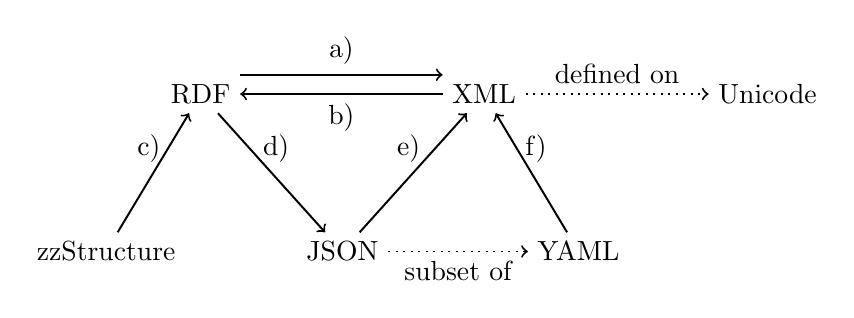
\begin{tikzpicture}[arrow/.style={draw,line width=0.25mm,->}]
\node (json) {JSON};
\node at (3,0) (yaml) {YAML};
\node at (-1.8,2) (rdf) {RDF};
\node at (1.8,2) (xml) {XML};
\node at (5.4,2) (unicode) {Unicode};
\node at (-3,0) (zzstruct) {zzStructure};
\draw[arrow] (rdf.north east) to node[above] {a)} (xml.north west);
\draw[arrow] (xml.west) to node[below] {b)} (rdf.east);
\draw[arrow] (zzstruct) to node[above] {c)~~} (rdf);
\draw[arrow] (rdf) to node[above] {~d)} (json);
\draw[arrow] (json) to node[above] {e)~~} (xml);
\draw[arrow,dotted] (json) to node[below] {subset of} (yaml);
\draw[arrow] (yaml) to node[above] {~f)} (xml);
\draw[arrow,dotted] (xml) to node[above] {defined on} (unicode);
\end{tikzpicture}
\begin{tabular}{ll}
a) & \term{RDF/XML}  \cite{Beckett2004} \\
b) & \term{RDF Schema} for \term{XML Infoset} \cite{Tobin2001} \\
c) & \term{zzStructure} in \acro{RDF} \cite{Gutteridge2010} \\
d) & \term{RDF/JSON} \cite{Alexander2008} \\
   & \term{JSON-LD} \cite{Sporny2012} \\
e) & \term{JSONx}    \cite{Muschett2011} \\
f) & \acro{YAML} in \acro{XML} \cite{BenKiki2006} \\
\end{tabular}
\caption{Existing encoding mappings between several data structuring languages}
\label{fig:jsonrdfxml}
\end{figure}

Given a set of precise mapping rules, any formal language can be encoded in, or
mapped to any other languages. To give some examples,
figure~\ref{fig:jsonrdfxml} shows existing encodings between \acro{JSON},
\acro{RDF}, \acro{XML}, and other \term{data structuring language}s. As the
mapping graph in figure~\ref{fig:jsonrdfxml} contains circles, one could
endlessly encode data in layers (RDF in RDF/XML in JSONx in XML Infoset in RDF
\ldots) without essentially adding value --- the existence of layers alone does
not guarantee that each layer actually hides complexity and details. In fact,
existing data can be compared with stratigraphic deposits in archaeology or
geology (see section~\ref{sec:dataarchaeology} for and extension of this
comparison). An example is \acro{MARCXML}, an encoding of \acro{MARC} in
\acro{XML} keeps irrelevant punctation and other artifacts from \term{ISBD} in
\acro{MARC}. In addition to full encodings that map every relevant aspect of
one language in another, there are abstractions which only cover a subset of
the original language. By this, a mapping can also be used as specification
(see section~\ref{sec:standardsrules}).

% \TODO{Add an example where XXX encoded in YYY does not fully cover all XXX}
% TODO: \term{unlimited semiosis}

Although each level of abstraction should fully hide the details of
implementation on levels below, one sometimes need to take into account several
levels, lacking a clean separation between each of them. An example is given by
\textcite{Thomale2010} for \acro{MARC}. The general reason why abstraction
cannot fully hide levels is the dependency on context. As ``abstraction is
deciding which aspects of a problem to consider and which ones to ignore''
\cite{Koenig1998} a specific abstraction only gives you one specific view to a
problem. Different views may be required for different applications. An
example of different views is given with the paradigms of documents and objects
in section~\ref{sec:docobj}.  A full separation of levels is also arguable from a
semiotic point of view: when one piece of data in language $A$ as sign refers
to another piece of data in language $B$ as object, the mode of reference is
not necessarily arbitrary: as showed by \person[Charles Sanders]{Peirce}, the
sign can also resemble the object (\term{iconic sign}), or the sign can
directly be connected to the object (\term{indexical sign}).  Examples of iconic
signs in data include grouping brackets and \term{descriptive identifier}s. 
Examples of indexical signs include pointers such as positions and hash codes
(section~\ref{sec:hashes}).  The iconic or indexical connection can also span
multiple levels of abstractions.

Although the paradigm of abstraction is omnipresent, applications and encoding
levels are often not known explicitly but concealed in the current use of
standards. For instance the division of markup in \term{procedural markup},
that describes what to do with a given data object, and \term{semantic markup},
that describes what a given data object is (section~\ref{sec:markuptypes})
depends on the level of description one chooses. As \textcite{Meek1995} puts it
in a nutshell ``one language's syntax can be another's semantics''\footnote{To
be honest, this interpretation of Meek may be against his intention as he only
tries to avoid the words `syntax' and `semantic'. The statement, however, gets
an additional meaning if one considers the stacking of multiple languages in
layers of abstraction. The term `language' in Meek's paper mainly refers to
\term{programming language}s but his results can also be applied to descriptive
data languages.} and ``most people will shift or mix levels without really
noticing that they are there at all''. This aspect of abstraction in levels has
been identified by \textcite{Eco1979} as an \term{unlimited semiosis}.  Meek,
in particular, stresses the importance of clearly distinguishing three levels
in language-independent modeling, which are listed in
table~\ref{tab:meekslevels}. In addition to the levels of data types
(section~\ref{sec:datatypes}) the levels of data modeling
(section~\ref{sec:datamodeling}) are most vital to this thesis.

\begin{table}
\center
\begin{tabular}{|l|l|}
\hline
\textbf{level} & \textbf{domain} \\
\hline
1) abstract & conceptual value space \\
2) computational  &  representable values and processes \\
\hspace{1em}a) linguistic/syntax  & how values are expressed \\
\hspace{1em}b) operational/semantic & processes which values express \\
3) representational & value representation \\
\hline
\end{tabular}
\caption{Levels of abstraction in language-independent standardization}
\label{tab:meekslevels}
\end{table}

A formal theory of abstraction within one method of description is provided by
\textcite{Keet2007,Keet2008c,Keet2011} as `\term{granularity}'. In Keets model
of granularity, different abstraction hierarchies can exist as parallel trees
(``perspectives'') that each partition a specific subject domain (a point of
view) according to specific properties. A simple example is the division of
documents in smaller parts or the partition of result sets by faceted browsing.
This theory or granularity has been applied to conceptual data models
\cite{Keet2007} and it can help to map multiple models that partly overlap on
different levels of description.

Independent of the kind of abstraction, each abstraction helps to focus on
particular properties, but it has a price: as expressed by \textcite{Yang2009}
``every abstraction layer does not only adds a little over head to the CPU, but
also to the poor human who has to read that code.'' Integration and readability
can be improved by redundancy and by precise standards (see
section~\ref{sec:standardsrules}). As standards can be fuzzy, violated, and
misinterpreted, there can be confusion about which which level of description
is actually used. For instance an \acro{RDF} document can use predicates from
the \acro{OWL} ontology, but this does not guarantee that the full enforcement
of owl-\term{entailment} with all of its aspects was actually intended. No
abstraction can fully remove the burden of actually reading and interpreting
digital documents.

\begin{description}
\item[Strength:] levels help to separate relevant and irrelevant parts.
\item[Weakness:] levels often cannot clearly be separated and too many
  levels may more confuse then they simplify.
\item[Patterns:] The pattern most likely found together with
  this paradigm include the \pattern{encoding} pattern and the
  \pattern{embedding} pattern.
\end{description}

